%\documentclass[pdflatex,11pt]{aghdpl}
\documentclass{aghdpl}               % przy kompilacji programem latex
% \documentclass[pdflatex,en]{aghdpl}  % praca w języku angielskim
\usepackage[polish]{babel}
\usepackage[cp1250]{inputenc}

% dodatkowe pakiety
\usepackage{enumerate}
\usepackage{listings}
\usepackage{amsmath}
\lstloadlanguages{TeX}

\lstset{
  literate={ą}{{\k{a}}}1
           {ć}{{\'c}}1
           {ę}{{\k{e}}}1
           {ó}{{\'o}}1
           {ń}{{\'n}}1
           {ł}{{\l{}}}1
           {ś}{{\'s}}1
           {ź}{{\'z}}1
           {ż}{{\.z}}1
           {Ą}{{\k{A}}}1
           {Ć}{{\'C}}1
           {�?}{{\k{E}}}1
           {Ó}{{\'O}}1
           {�?}{{\'N}}1
           {�?}{{\L{}}}1
           {Ś}{{\'S}}1
           {Ź}{{\'Z}}1
           {Ż}{{\.Z}}1
}

%---------------------------------------------------------------------------

\author{Jakub Gola\\ Zbigniew Tekiela}
\shortauthor{J.Gola, Z.Tekiela}

\titlePL{Metody inicjalizacji modelu t{\l{}}a}
\titleEN{Background model initialisation methods}

\shorttitlePL{Metody inicjalizacji modelu t{\l{}}a} % skrócona wersja tytułu jeśli jest bardzo długi
\shorttitleEN{Background model initialisation methods}

\thesistypePL{Praca in{\.z}ynierska}
\thesistypeEN{Bachelor of Science Thesis}

\supervisorPL{dr hab. Marek Gorgo{\'n}}
\supervisorEN{Marek Gorgo{\'n} Ph.D}

\date{2012}

\departmentPL{Katedra Automatyki}
\departmentEN{Department of Automatics}

\facultyPL{Wydzia{\l{}}� Elektrotechniki, Automatyki, Informatyki i In{\.z}ynierii Biomedycznej}
\facultyEN{Faculty of Electrical Engineering, Automatics, Computer Science and Biomedical Engineering}

\acknowledgements{Serdecznie dzi{\k{e}}kuj{\k{e}}.}



\setlength{\cftsecnumwidth}{10mm}

%---------------------------------------------------------------------------

\begin{document}

\titlepages

\tableofcontents
\clearpage

\chapter{Metody operuj�ce na poziomie pikseli}
\label{cha:Metody operuj�ce na poziomie pikseli}
\section{Mixture of Gaussians (MOG)}
\subsection{Wprowadzenie}
T�o sceny zawiera wiele dynamicznych obiekt�w jak poruszane na wietrze ga��zie i~li�cie drzew czy krzew�w. Zmiany w~obrazie nimi wywo�ane powoduj�, �e warto�� intensywno�ci danego piksela oraz jego kolor w~czasie mog� si� bardzo r�ni� od siebie. Z~tego powodu wykorzystanie pojedynczego przybli�enia rozk�adu prawdopodobie�stwa przy u�yciu krzywej Gaussa daje z�e rezultaty. Zamiast tego w~opisywanej metodzie u�yto podej�cia bazuj�cego na wykorzystaniu kilku rozk�ad�w Gaussa o~r�nych parametrach w~celu zamodelowania takich zmian \cite{7}.

Standardowe adaptacyjne modele t�a polegaj� na tworzeniu aproksymacji t�a, kt�re jest podobne do obecnej statycznej sceny za wyj�tkiem miejsc, w~kt�rych odby� si� ruch. Podej�cie takie jest efektywne w~sytuacjach, gdy obiekty poruszaj� si� stale, a~t�o jest widoczne znaczn� cz�� czasu, jednak�e nie sprawdza si� ono dla scen zawieraj�cych du�o poruszaj�cych si� obiekt�w, a~w szczeg�lno�ci, gdy obiekty te poruszaj� si� powoli. Nie potrafi tak�e poradzi� sobie z~t�ami posiadaj�cymi rozk�ad dwumodalny, powoli odtwarza t�o je�li zostanie ono odkryte i~ma jeden ustalony pr�g dla ca�ej sceny. 

W metodzie MOG zamiast modelowa� warto�ci wszystkich pikseli jako wy��cznie jeden typ rozk�adu, modelowane s� one mieszank� rozk�ad�w Gaussa. Bazuj�c na wadze i~wariancji ka�dego u�ytego do mieszanki rozk�adu Gaussa okre�lane jest, kt�re z~nich mog� odnosi� si� do kolor�w t�a. Warto�ci pikseli, kt�re nie mieszcz� si� w~�adnym rozk�adzie t�a uznawane s� za piksele nale��ce do pierwszego planu. Taki stan pikseli utrzymuje si� do czasu kiedy zaczn� wystarczaj�co dobrze pasowa� do kt�rego� z~rozk�ad�w t�a. 

Opisywana metoda dostosowuje si� aby radzi� sobie ze zmianami o�wietlenia, powtarzalnymi ruchami element�w t�a, powolnie poruszaj�cymi si� elementami pierwszego planu oraz wprowadzaniu lub usuwaniu element�w ze sceny. Powolnie poruszaj�ce si� elementy potrzebuj� wi�cej czasu aby wpasowa� si� w~t�o, poniewa� rozk�ad do kt�rego pasuj� ma wi�ksz� wariancj� ni� t�o. Powtarzaj�ce si� zmiany r�wnie� s� uwzgl�dniane, a~model rozk�adu t�a jest utrzymywany nawet je�li jest chwilowo zamieniony przez inny rozk�ad, co prowadzi do szybszego odtworzenia t�a w~przypadku usuni�cia obiekt�w ze sceny.
Metoda ta wykorzystuje dwa podstawowe parametry: 
\begin{lstlisting}
a - sta�a uczenia
T - porcja danych jaka powinna by� uwzgl�dniona w~tle
\end{lstlisting}

Zak�adaj�c, �e ka�dy piksel obrazu b�dzie pochodzi� z~jednej p�aszczyzny przy zmiennym �wietleniu, to do wydzielenia t�a z~takiego obrazu wystarczy u�ycie pojedynczej adaptacyjnej aproksymacji rozk�adem Gaussa dla ka�dego piksela. Jednak�e w~rzeczywistych warunkach na obrazie wyst�puje wiele powierzchni oraz zmienne o�wietlenie, co sprawia, �e potrzebne staje si� u�ycie kilku adaptacyjnych rozk�ad�w Gaussa. W~opisywanej metodzie u�yta jest mieszanka kilku takich rozk�ad�w o~r�nych parametrach. Za ka�dym razem, gdy parametry rozk�adu s� aktualizowane, nast�puje proces oceny dost�pnych rozk�ad�w w~celu okre�lenia tego najbardziej prawdopodobnego. 

\subsection{Opis metody}
\subsubsection{Model mieszanki}

Niech kolejne warto�ci danego piksela w~czasie nazywaj� si� histori� piksela. Zatem historia piksela jest to seria warto�ci danego piksela, gdzie dla obraz�w w~skali szaro�ci s� to warto�ci skalarne, a~dla obraz�w kolorowych s� to wektory. O~danym pikselu $\{x_0,y_0\}$ w~danej chwili czasu t, mo�na powiedzie�, �e znana jest jego historia
\begin{equation}
\{X_1,\dots,X_t\}=\{I(x_0,y_0,i):1\le i \le t\}
\end{equation}
gdzie $I$ jest sekwencj� ramek.

Niedawna historia dla ka�dego piksela modelowana jest mieszank� K~rozk�ad�w Gaussa. Prawdopodobie�stwo zaobserwowania obecnego piksela okre�la si� wzorem

\begin{equation}
P(X_t)=\sum_{i=1}^{K} \omega_{i,t} * \eta(X_t, \mu_{i,t} , \Sigma_{i,t})
\end{equation}

\noindent gdzie K~jest liczb� rozk�ad�w,  $\omega_{i,t}$ jest oszacowan� wag� $i$-tego rozk�adu w~mieszance w~chwili $t$, $\mu_{i,t}$ jest �redni� warto�ci�  $i$-tego rozk�adu w~mieszance w~chwili $t$, $\Sigma_{i,t}$ jest macierz� kowariancji w~chwili $t$,$\eta$ jest funkcj� g�sto�ci prawdopodobie�stwa Gaussa:

\begin{equation}
\eta(X_t,\mu,\Sigma)=\frac{1}{(2\pi)^\frac{n}{2} |\Sigma|^\frac{1}{2}}e^{-\frac{1}{2}(X_t-\mu_t)^T \Sigma^{-1} (W_t -\mu_t)}
\end{equation}

\noindent gdzie K~okre�lane jest przez dost�pn� pami�� oraz moc obliczeniow� jednostki na kt�rej wykonywany jest algorytm. Najcz�ciej spotykana warto�� mie�ci si� w~zakresie od 3~do 5. W~celu zmniejszenia ilo�ci oblicze� przyjmuje si�, �e macierz kowariancji ma posta�:

\begin{equation}
\Sigma_{k,t}=\sigma^2_kI
\end{equation}

Takie rozwi�zanie zak�ada, �e warto�ci dla poszczeg�lnych sk�adowych barwnych ka�dego piksela maj� tak� sam� wariancj�. Za�o�enie to obci��one jest pewnymi b��dami, lecz pozwala unikn�� wykonywania operacji odwracania macierzy, co jest zadaniem bardzo kosztownym, za cen� mniejszej precyzji. 

Zatem rozk�ad ostatnio obserwowanych warto�ci dla ka�dego piksela w~obrazie opisany jest mieszank� rozk�ad�w Gaussa. Nowa warto�� piksela b�dzie na og� reprezentowana przez jeden z~g��wnych sk�adnik�w mieszanki. 

Do obliczenia warto�ci nowego piksela u�yta zosta�a metoda on-line K-means approximation. Ka�da warto�� piksela jest sprawdzana pod k�tem dopasowania do jednego z~K rozk�ad�w. Warunkiem przynale�no�ci jest warto�� w~zakresie do 2,5 odchylenia standardowego z~danego rozk�adu. Zmiana opisanego wcze�niej progu ma niewielki wp�yw na wydajno�� algorytmu. Opisany spos�b wyboru odpowiednich pikseli jest bardzo u�yteczny dla obszar�w z~r�nym o�wietleniem, poniewa� obiekty znajduj�ce si� w~zacienionych obszarach maj� mniejszy szum ni� obiekty znajduj�ce si� w~ja�niejszych regionach.

W przypadku, gdy �aden rozk�ad nie zosta� dopasowany do danego piksela, to rozk�ad z~najmniejsz� wag� jest zast�powany nowym z~warto�ci� piksela jako now� warto�ci� oczekiwan�, du�� wariancj� i~nisk� wag�.

Wcze�niejsze wagi K~rozk�ad�w w~czasie t~s� aktualizowane wg wzoru: 

\begin{equation}
\omega_{k,t}=(1-\alpha)\omega_{k,t-1}+\alpha(M_{k,t})
\end{equation}
gdzie: $\alpha$ to tempo uczenia, a~$M_{k,t}$ jest 1~dla dopasowanego rozk�adu i~0 dla pozosta�ych rozk�ad�w. Po dokonaniu aproksymacji wagi s� normalizowane. $\frac{1}{\alpha}$ oznacza sta�� czasow� okre�laj�c� pr�dko�� z~jak� parametry rozk�ad�w si� zmieniaj�.

Dla rozk�ad�w niedopasowanych do danego piksela warto�ci $\mu$ i~$\sigma$ pozostaj� niezmienione. Dla rozk�ad�w, kt�re zosta�y dopasowane warto�ci $\mu$ i~$\sigma$ obliczane s� nast�puj�co:

\begin{equation}
\mu_t=(1-\rho)\mu_{t-1}+\rho X_t
\end{equation}

\begin{equation}
\sigma^2_t=(1-\rho)\sigma^2_{t-1}+\rho(X_t-\mu_t)^T(X_t-\mu_t)
\end{equation}
przy czym:

\begin{equation}
\rho = \alpha\eta(X_t|\mu_k,\sigma_k)
\end{equation}

Jedn� z~najwi�kszych zalet opisanego rozwi�zania jest fakt, �e kiedy jaki� obiekt zostanie dodany do t�a, to nie niszczy on istniej�cego modelu t�a. Oryginalny kolor t�a zostaje zachowany w~mieszance do czasu, a� stanie si� najmniej prawdopodobnym kolorem oraz zostanie zaobserwowany nowy kolor. Zatem je�li obiekt pozostanie nieruchomy wystarczaj�co d�ugo aby sta� si� cz�ci� t�a, a~nast�pnie si� poruszy, to rozk�ad opisuj�cy poprzednie t�o ci�gle istnieje w~tymi samymi $\mu$ i~$\sigma^2$, ale mniejszym $\omega$ przez co mo�e zosta� szybko ponownie do��czony do modelu t�a.

\subsubsection{Estymacja modelu t�a}


Podczas gdy parametry modelu mieszanki dla ka�dego piksela zmieniaj� si�, nale�y okre�li� kt�re rozk�ady z~mieszanki daj� najwi�ksze prawdopodobie�stwo bycia wygenerowanymi przez procesy t�a. Z~heurystycznego punktu widzenia najbardziej interesuj�ce s� rozk�ady, kt�re daj� najlepsze dopasowanie i~najmniejsz� wariancj�


W celu wybrania odpowiednich rozk�ad�w nale�y uszeregowa� je wed�ug warto�ci $\omega$/$\sigma$. Warto�� ta ro�nie zar�wno przy zwi�kszeniu dopasowania, jak i~przy zmniejszeniu wariancji. W~praktyce tak uszeregowana lista daje zbi�r rozk�ad�w, gdzie najbardziej prawdopodobni kandydaci znajduj� si� na pocz�tku, a~najmniej prawdopodobni na ko�cu.
Selekcji pierwszych rozk�ad�w do modelu t�a dokonuje si� za pomoc� wzoru 

\begin{equation}
B = argmin_b\left(\sum_{k=1}^{b}\omega_k>T\right)
\end{equation}
gdzie: T~jest miar� minimalnej ilo�ci danych jaka powinna by� prana pod uwag�. Rozwi�zanie takie bierze pod uwag� najlepiej dostosowany rozk�ad dot�d, a� pewna porcja T~danych jest rozwa�ona. Je�li T~jest jest warto�ci� ma��, to tedy model t�a zazwyczaj jest unimodalny. Je�li T~jest warto�ci� wi�ksz�, multimodalny rozk�ad wywo�any powtarzalnymi ruchami w~tle mo�e skutkowa� uwzgl�dnieniem w~modelu t�a wi�cej ni� jednego koloru. Skutkuje to efektem przezroczysto�ci, kt�ry pozwala modelowi przyjmowa� dwa lub wi�cej oddzielnych kolor�w. 


\section{�rednia z~bufora ramek}
\subsection{Wprowadzenie}
�rednia z~bufora ramek jest jedn� z~najprostszych mo�liwych metod generacji t�a. Algorytm ten opiera si� na wyliczaniu �redniej arytmetycznej dla ka�dej pozycji piksela na obrazie spo�r�d ramek zgromadzonych w~buforze.

\subsection{Opis metody}
Warto�� dla ka�dego piksela t�a wyliczana jest ze wzoru.

\begin{equation}
B(x,y)=\frac{1}{n} \sum_{i=1}^{n} P(x_i,y_i)
\end{equation}

\noindent Gdzie: $B(x,y)$ oznacza obecn� warto�� piksela t�a w~miejscu (x,y), $n$ oznacza rozmiar bufora, $P(x_i,y_i)$ oznacza warto�� piksela na pozycji (x,y) w~$i$-tej ramce w~buforze.


\section{Aproksymacja �redniej przy u�yciu parametru alfa}
\subsection{Wprowadzenie}

Metoda ta jest modyfikacj� �redniej z~bufora ramek. Jej g��wnym za�o�eniem jest aproksymacja �redniej za pomoc� morfingu ramek. Daje ona podobne rezultaty, jednak�e w~przeciwie�stwie do swojego pierwowzoru nie wykorzystuje bufora, a przez to charakteryzuje si� mniejsz� z�o�ono�ci� pami�ciow�.

\subsection{Opis metody}
Warto�� dla ka�dego piksela t�a wyliczana jest ze wzoru.

\begin{equation}
\label{alpha}
B_{n}(x,y) = P_{n}(x,y) * \alpha + B_{n-1}(x,y) * (1-\alpha)
\end{equation}

\noindent gdzie $B_{n}(x,y)$ oznacza obecn� warto�� piksela t�a w~miejscu (x,y), $P_{n}(x,y)$ oznacza warto�� piksela na pozycji (x,y) w~obecnej ramce, $B_{n-1}$ oznacza warto�� piksela na pozycji (x,y) w~poprzednim modelu t�a

\include{rozdzial3}
\chapter{S�ownik u�ytych poj��}
\label{slownik}

\begin{description}
\item[inicjalizacja t�a] proces jednorazowy, w kt�rym na podstawie pewnej ilo�ci ramek i odpowiednich algorytm�w zostaje uzyskany model t�a
\item[generecja t�a] ci�g�y proces aktualizacji wst�pnie zainicjalizowanego modelu  t�a
\item[blok] wydzielona kwadratowa cze�� ramki o~rozmiarach $N*N$, zawieraj�ca opr�cz pikseli informacj� o~wadze superbloku
\item[superblok] grupa 4~s�siaduj�cych ze sob� blok�w, tworz�ca wi�kszy blok(superblok) o~rozmiarach $2N * 2N$
\begin{figure}[ht]
\begin{center}
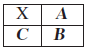
\includegraphics{blok.png}
\caption{Blok X~oraz jego otoczenie, tworz�ce razem z~nim superblok}
\end{center}
\end{figure}  
\item[grupa kandydat�w]
\item[lokalizacja blokowa]
\end{description}

% itd.
% \appendix
% \chapter{Dodatek A - spis zawarto�ci p�yty CD}

Do niniejszej pracy zosta�a do��czona p�yta CD zawieraj�ca foldery:
\begin{description}
\item[praca] - praca w formacie pdf
\item[praca\_latex] - praca w formacie \LaTeX
\item[sekwencje] - sekwencje u�yte do bada�
\item[kod] - kody �r�d�owe program�w napisanych w ramach pracy
\end{description}
% \chapter{Dodatek B - opis informatyczny programu}

W ramach niniejszej pracy zosta�y wykonane 2 programy napisane w j�zyku C++ przy u�yciu biblioteki OpenCV.
\section{Program robust}
Program \textbf{robust.exe} zawiera w sobie implementacj� 2 algorytm�w. S� nimi algorytm MOG oraz blokowy (przestrzenny), kt�ry w zale�no�ci od parametr�w wej�ciowych u�ywa transformaty Hadamarda lub DCT. 

Program ten przyjmuje parametry wej�ciowe w nast�puj�cej kolejno�ci:

\begin{enumerate}
\item �cie�ka do analizowanej sekwencji wideo,
\item wielko�� bufora ramek,
\item u�ywana metoda: 0 - MOG, 1 - metoda wykorzystuj�ca transformat� DCT, 2 - metoda wykorzystuj�ca transformat� Hadamarda,
\item rozmiar bloku (w przypadku wybrania metody MOG parametr ten pomija si�),
\item wsp�czynnik $T_{corr}$ (w przypadku wybrania metody MOG parametr ten pomija si�),
\item wsp�czynnik $T_{mad}$ (w przypadku wybrania metody MOG parametr ten pomija si�).
\end{enumerate}
Program sk�ada si� z nast�puj�cych klas
\subsection{blok}
Klasa blok przechowuje w kontenerze typu vector zawarto�� pojedynczego bloku. Posiada ona r�wnie� zmienn� weight, reprezentuj�c� wag� bloku oraz size, okre�laj�c� jego rozmiar. Jej najwa�niejsze metody to:
\begin{enumerate}
\item int getSize() - zwraca rozmiar bloku,
\item double mean() - oblicza �redni� z pikseli wchodz�cych w sk�ad bloku,
\item double deviation() - oblicza odchylenie standardowe z pikeli wchodz�cych w sk�ad bloku,
\item double corelation(blok \&blk) - oblicza wsp�czynnik korelacji z innym blokiem,
\item double mad(blok \&blk) - oblicza wsp�czynnik MAD z innym blokiem,
\item boolean similar(blok \&blk, double T1,double T2) - zwraca prawd�, je�li blok jest podobny do innego bloku przy wsp�czynniku korelacji r�wnym T1 i wsp�czynniku MAD r�wnym T2.
\end{enumerate}
\subsection{grid}
Klasa grid przechowuje ca�� siatk� grupy kandydat�w. Jej najwa�niejsze metody to:
\begin{enumerate}
\item void insertAt(int x,int y, blok\&) - wstawia do grupy kandydat�w dla lokalizacji blokowej o wsp�rz�dnych $(x,y)$ blok blk,
\item grid(int \_width, int \_height) - konstruktor, ustawiaj�cy wysoko�� i szeroko�� siatki,
\item void reserve(int n) - rezerwuje w pami�ci obszar do stworzenia siatki mog�cej pomie�ci� n element�w, musi by� wywo�ana po stworzeniu obiektu typu grid,
\item void fix() - naprawia b��dy zwi�zane z nieprawid�owo�ciami podczas przechwytywania obrazu (usuwa nieprawid�owe bloki z siatki) - musi by� wywo�ana po zako�czeniu kolekcjonowania kandydat�w.
\end{enumerate} 
\subsection{background}
Klasa background przechwouje odtworzone fragmenty t�a w kontenerze typu vector. Zawiera r�wnie� tablic� int**filltable, okre�laj�c�, czy dana lokalizacja blokowa posiada ju� odtworzone t�o (je�li tak, w tablicy w miejscu o wsp�rz�dnych x i y b�dzie znajdowa� si� warto�� 1) oraz licznik int nrfilled okre�laj�cy, ile fragment�w t�a zosta�o ju� odtworzonych. 
jej najwa�niejsze metody to:
\begin{enumerate}
\item Mat \& devectorize() - zwraca t�o jako obiekt Mat, kt�ry mo�na zapisa� i wy�wietli� przy u�yciu standardowych funkcji OpenCV,
\item void insertAt(int x,int y, blok\&) - wstawia dla lokalizacji blokowej o wsp�rz�dnych $(x,y)$ dany blok,
\item int isFilled(int x,int y) - zwraca ,,1'' gdy dla danej lokalizacji blokowej t�o zosta�o ju� odtworzone.
\end{enumerate}
\subsection{utils}
Utils jest klas� pomocnicz�, zawieraj�c� nast�puj�ce funkcje:
\begin{enumerate}
\item Mat** grid\_cut(Mat input\_image, int size) - zwraca ramk� obrazu w postaci tablicy obiekt�w Mat o danym rozmiarze - innymi s�owy dzieli j� na ma�e fragmenty,
\item - double cost(Mat C, Mat D,int size, double alpha, int weight) - liczy funkcj� kosztu dla transformaty, zgodnie ze wzorem (\ref{costfun}),
\item Mat hadamardmat(int size) - zwraca obiekt Mat b�d�cy macierz� Hadamarda o zadanym rozmiarze.
\end{enumerate}
\subsection{robust}
Robust jest to g��wna klasa, wykonuj�ca obliczenia na sekwencjach wideo i zwracaj�ca obrazy wynikowe t�a. Po uruchomieniu,gdy zostanie wywo�ana dla metod blokowych, tworzy ona pojedyncze obiekty klas grid(do przechowywania grupy kandydat�w) i background (do przechowywania odtworzonego t�a), a nast�pnie przetwarza ka�d� kolejn� ramk� zgodnie z algorytmem opisanym w sekcji \ref{blo:algorytm}. W przypadku wywo�ania jej dla metody MOG, u�ywa ona wbudowanej w OpenCV klasy BackgroundSubtractorMOG2, pozwalaj�cej obliczy� model t�a metod� MOG.
\section{Program simple\_pixel\_methods} 
Program \textbf{simple\_pixel\_methods.exe} zawiera w sobie implementacj� 3 algorytm�w. S� nimi algorytmy: �redniej z bufora, aproksymacji �redniej z bufora oraz mediany.

Program ten przyjmuje parametry wej�ciowe w nast�puj�cej kolejno�ci:

\begin{enumerate}
\item wielko�� bufora ramek,
\item typ metody (0 - aproksymacja, 1 - �rednia, 2 - mediana),
\item warto�� parametru $\alpha$ w przypadku wybrania metody aproksymacji.
\end{enumerate}

nie wiem co tu dalej napisa�...
% itd.

\bibliographystyle{alpha}
\bibliography{bibliografia}
%\begin{thebibliography}{1}
%
%\bibitem{Dil00}
%A.~Diller.
%\newblock {\em LaTeX wiersz po wierszu}.
%\newblock Wydawnictwo Helion, Gliwice, 2000.
%
%\bibitem{Lam92}
%L.~Lamport.
%\newblock {\em LaTeX system przygotowywania dokumentów}.
%\newblock Wydawnictwo Ariel, Krakow, 1992.
%
%\bibitem{Alvis2011}
%M.~Szpyrka.
%\newblock {\em {On Line Alvis Manual}}.
%\newblock AGH University of Science and Technology, 2011.cccccc
%\newblock \\\texttt{http://fm.ia.agh.edu.pl/alvis:manual}.
%
%\end{thebibliography}

\end{document}
